\section{Evaluation}
The purpose of selective decoding is to achieve more efficient zoomable video playback. We evaluate the efficiency of selective decoding from two aspects, video playback frame rate and energy consumption. 

We used two test phones for evaluation with the specifications shown below.
\begin{table}
\centering
\caption{Test Phones for Evaluation}
\begin{tabular}{|p{2.0cm}|p{2.0cm}|p{1.5cm}|p{2.0cm}|p{2.0cm}|p{1.5cm}|}
\hline
Phones & CPU Clock Rate & RAM & CPU Info & Display & Android Version \\
\hline
HTC Incredible S & 1GHz & 768MB & ARMv7 rev1, with NEON & S-LCD, 480x800 & 2.3.7 \\
\hline
Samsung Galaxy S2 & Dual Core 1200 MHz & 1024 MB & ARMv7 rev1, with NEON & Super Amoled Plus 480x800 & 2.3.6 \\
\hline
\end{tabular}
\end{table}
The description thereafter refers HTC Incredible S as Phone A, and Samsung Galaxy S2 as Phone B.

Two test video sequences are used for evaluation. The first video sequence is a lecture recording with little motion, and the second video sequence contains constnt object motion. Both videos are 1080p HD videos. We refer them as video sequence 1 and video sequence 2 respectively in subsequent description.

\subsection{Frame Rate}
Video playback frame rate is affected by both ROI sizes and ROI positions. We test the influence of each. We also measure the overhead by selective decoding in terms of frame rate. All the test for frame rate are done three times and the average value is recorded for analysis. 

\subsubsection{Different ROI Positions}
Different regions of a video frame may contain different amount of motions and dependencies, therefore the ROI position can affect the amount of processing at decoding and subsequently the video playback frame rate. 

We fix the ROI size, and then move the ROI from the upper left corner to the lower right of the video frame. 
%This is shown as figure below,
%\begin{figure}
%\centering
%\vspace{2.5cm}
%\includegraphics[height=2.5cm]{roip.eps}
%\subfigure{\includegraphics[height=1.7cm]{pos1.eps}}
%\subfigure{\includegraphics[height=1.7cm]{pos2.eps}}
%\subfigure{\includegraphics[height=1.7cm]{pos3.eps}}
%\subfigure{\includegraphics[height=1.7cm]{pos4.eps}}
%\caption{ROI of 2x2 at Different Positions}
%\end{figure}

%The figure above shows a ROI of 2x2 macroblocks in a video frame of 6x4 macroblocks. The figure shows four possible positions of the ROI. Starting from the position at figure ?(a), we move the ROI to the right until the right side of the ROI reaches the right side of the frame. We also move the ROI down to the bottom as shown in figure ?(d).

The test are carried out for three different ROI sizes, with the ROI width and height set as 50\%, 70\%, and 90\% of the original video's width and height. Below are the results,
\begin{figure}
\centering
%\subfigure[Phone A Video 1]{\includegraphics[height=4.0cm]{fr1a1.eps}}
%\subfigure[Phone A Video 2]{\includegraphics[height=4.0cm]{fr1a2.eps}}
%\\
\subfigure[Phone B Video 1]{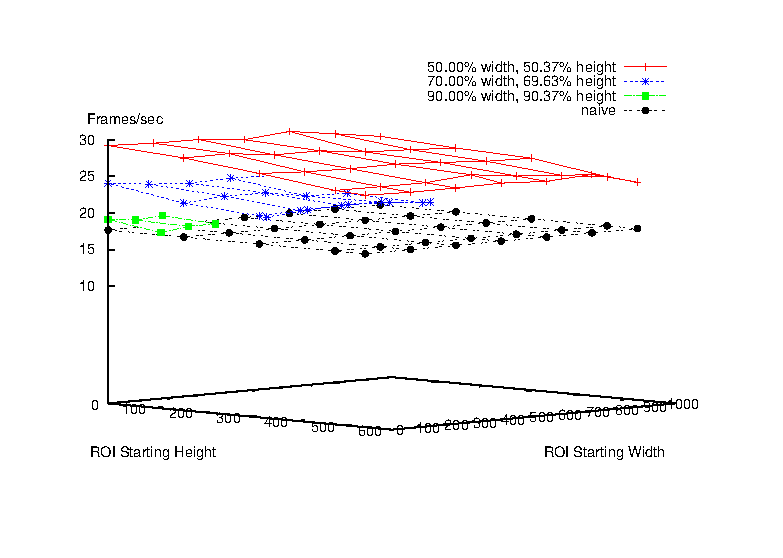
\includegraphics[height=4.0cm]{fr1b1.eps}}
\subfigure[Phone B Video 2]{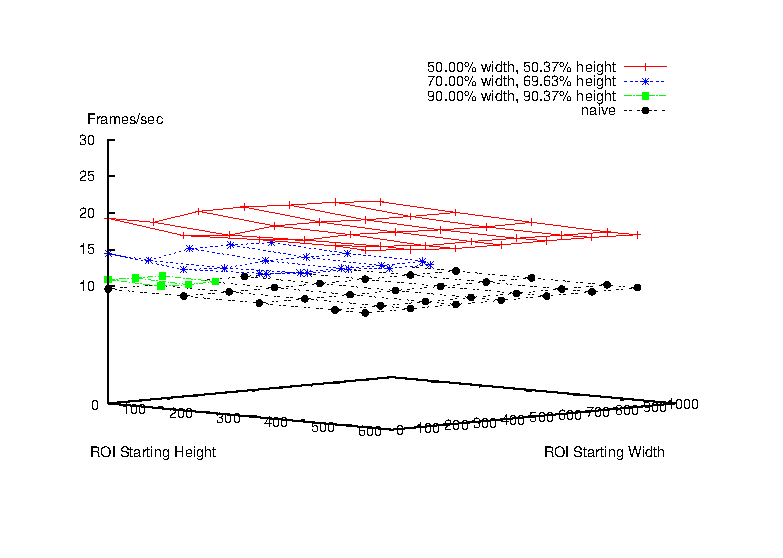
\includegraphics[height=4.0cm]{fr1b2.eps}}
\caption{Frame Rate with 90\%, 70\%, and 50\% of ROI at Different Positions}
\end{figure}
In figures above, each 3D interface indicatest the frame rate for a ROI size. The intersection in a surface indicate the start position of a particular ROI size. 

Looking at a single 3D interface at each figure, the frame rate tends to decrease when ROI starting witdth and/or starting height increases. This is because the intra-VOP dependencies increases towarding the lower right, and more dependencies cause more macroblocks to be selected and decoded, and thus the frame rat decreases. However, there are exceptions to this decrease trend, which are probably caused by different amount of motions and motion dependencies at different ROI positions. 

Compare different 3D interfaces at a single figure, it is clear that the ROI size has a more significant effect than ROI positions. At 3 out of 4 test combinations, when ROI size is smaller than 90\%, the frame rate of selective decoding is higher than standard MPEG4 SP decoding. 

Compare figures for a single phone, the frame rate for video sequence 1 is higher than video sequence 2. This is expected because video sequence 1 has less amount of motion than video sequence 2. Compare figures for a single video sequence, the frame rate for phone A is lower than phone B. This is because phone B has more powerful hardware. 

\subsubsection{Different ROI Size}
Previous test already reveals that ROI size has significant influcence on video playback frame rate at selective decoding. This experiment examines the affection of ROI size more closely. We position the ROI at the center of the video frame and vary the ROI height and width from 10\% to 100\% of original video height and width. Below shows the experiment results,
\begin{figure}
\centering
%\subfigure[Phone A Video 1]{\includegraphics[height=2.0cm]{fr2a1.eps}}
%\subfigure[Phone A Video 2]{\includegraphics[height=2.0cm]{fr2a2.eps}}
\subfigure[Phone B Video 1]{\includegraphics[height=3.0cm]{fr2b1.eps}}
\subfigure[Phone B Video 2]{\includegraphics[height=3.0cm]{fr2b2.eps}}
\caption{Frame Rate with 10\% to 100\% ROI Centered}
\end{figure} 
Looking at each figure, frame rate decreases as ROI size increases. At figure ??, selective decoding achieves higher frame rate at ROI size at around 80\% or less. At the rest of the figures, selective decoding decodes faster at ROI size smaller than 90\%. At 10\% ROI, the frame rate on phone A is improved by 57.5\% for video sequence 1, and 237.7\% for video sequence 2, while the frame rate on phone B is improved by 76.3\% and 193.3\% respectively.  

Compare figures for a single phone or a single video, we can draw similar conclusions to the ROI position experiment. In addition, the curves at different figures differ due to different amount of motion at center of the video frame and ifferent phone processing capabilities. 

\subsubsection{Selective Decoding Overhead}
To evaluate the overhead of selective decoding, we set the ROI as the entire video frame. 
\begin{table}
\caption{Full Frame Selective Decoding VS. Standard Decoding}
\centering
\begin{center}
\begin{tabular}{|p{1.5cm}|p{1.5cm}|p{1.5cm}|p{1.5cm}|p{1.5cm}|}
\hline
Decoding Methods & Phone A Video 1 & Phone A Video 2 & Phone B Video 1 & Phone B Video 2 \\
\hline
Selective Decoding  &  10.57  &   6.30  &  16.81  &  9.60\\
%\hline
Standard Decoding   &  11.82  &   6.50  &  17.67  &  9.73 \\
\hline
\end{tabular}
\end{center}
\end{table}

Because of selective mask computation, selective decoding has lower playback frame rate than standard decoding. The overhead, however, is not signficant. In the four test combinations, the overhead is 10.58\%, 3.08\%, 4.87\%, and 1.34\% respectively. In practice, we can switch between selective decoding and standard decoding dynamically based on ROI sizes to achieve higher frame rate. 

In summary, the experiments show that selective decoding can effectively increase frame rate at ROI sizes around 80\%~90\% or less. 
 
\subsection{Energy Consumption} 
Energy consumption is the other important asepct of our evaluation. Two experiments are done with different focus. The first experiment utilizes a third-party Android application PowerTutor[Zhang:2010:AOP:1878961.1878982] to measure the power consumption at hardware component level. The second experiment measures the percentage of battery power discharged when playing the two different video sequences repeatedly for certain number of times. 

\subsubsection{PowerTutor Measurements}
Battery energy is mainly consumed by display and CPU at video playback. PowerTutor, an Android power measurement tool, is capable of measuring power consumed by different hardware components of a specific app. In the experiment, we vary the ROI sizes from 10\% to 100\%. The frame rate is controlled so that both selective decoding and standard decoding always play at same frame rate. This is mainly because the CPU display power is dependent on time and display content and controlling the time is essential for a fair comparison. Each test is done three times and the average value is recorded. 

For display measurements, we found the curves for selective decoding and standard decoding almost overlap, which means they consume similar amount of energy. However, this is not the case for CPU power consumption, which are shown as below. 
\begin{figure}
\centering
%\subfigure[Phone A Video 1]{\includegraphics[height=2.0cm]{pta1.eps}}
%\subfigure[Phone A Video 2]{\includegraphics[height=2.0cm]{pta2.eps}}
\subfigure[Phone B Video 1]{\includegraphics[height=3.0cm]{ptb1.eps}}
\subfigure[Phone B Video 2]{\includegraphics[height=3.0cm]{ptb2.eps}}
\caption{CPU Power Consumption Per Frame}
\end{figure}
Looking at each figure individually, CPU power consumption per frame at selective decoding increases when ROI size increases. At ROI size 90\% or less, CPU power consumption at selective decoding is lower than standard decoding at all four test combinations. At figure ???, selective decoding has lower power consumption at 100\%, this is probably because the MV decoding and DC\&AC prediction coding avoided by selective decoding online computation weigh more than selective mask computation, which is the overhead due to selective decoding.

Compare figures for a single phone, video playback for video with heavy motion tends to consume more power because of more motion compensation decoding. Selective decoding tends to save more energy for the heavy motion video by reducing number of macroblocks decoded, and subsequently amount of motion compensation decoding. 

Compare figures for a single video sequence, the amount of energy consumed by different phones differ. This is probably due to different hardware specifications. 

The overall power consumption measurements follow the similar trend as CPU power consumption, therefore it is not shown here. 

\subsubsection{Power Drain Experiment}
PowerTutor measurments show selective decoding can save energy, mainly by reducing CPU power consumption. However, PowerTutor measurement is obtained through offline-training models\cite{Zhang:2010:AOP:1878961.1878982} and may not be accurate for all phones. In addition, the measurements does not take into RAM and SDCARD access into consideration. 

We designed and carried out another experiment to measure the power consumption. In this experiment, we place ROI of different sizes at the video frame center and play the video repeatedly for certain number of times while keeping the frame rate same for a single test combination. Based on the processing power and video sequence, we set the frame rate for phone A as 9 FPS and 6FPS, and frame rate for phone B as 15 FPS and 8FPS. The percentage of power drained is recorded for comparison. Before each test, we fully charge the phone battery to 100\% and disable all background acitities including WiFi, Bluetooth, GPS, etc. All tests are repeated twice and the average is taken for plotting the graphs below,
\begin{figure}
\centering
%\subfigure[Phone A Video 1]{\includegraphics[height=2.0cm]{pwa1.eps}}
%\subfigure[Phone A Video 2]{\includegraphics[height=2.0cm]{pwa2.eps}}
\subfigure[Phone B Video 1]{\includegraphics[height=3.0cm]{pwb1.eps}}
\subfigure[Phone B Video 2]{\includegraphics[height=3.0cm]{pwb2.eps}}
\caption{Percentage of Power Drained}
\end{figure}
Looking at each figure individually, it is clear that selective decoding consumes less power when ROI sizes are below certain size. At 10\% ROI size, the battery consumption on phone A is reduced by 27.8\% and 24.8\% for video sequence 1 and 2 respectively, while the battery consumption on phone B is reduced by 61.1\% and 64.5\%. Because we set the frame rate differently for different phones and video sequences, the comparison for different phones and video sequences are not fair and therefore avoided. 

In summary, selective decoding proves to be efficient in terms of achiving higher frame rate and saving battery energy consumption when ROI size is below certain threshold.  




